\documentclass[a4paper,review,12pt,authoryear]{elsarticle}

\usepackage{natbib}
\usepackage{amsfonts,amsmath,bm,xcolor, booktabs,hyperref}
\usepackage[ruled]{algorithm2e}
\usepackage{geometry}
\usepackage{subfig}
\geometry{a4paper,scale=0.8}
\usepackage{setspace}
\setstretch{1.5}
\let\code=\texttt
\let\proglang=\textsf
\setcounter{MaxMatrixCols}{20}


\newcommand{\bY}{\mathbf{Y}}
\newcommand{\bpi}{\bm{\pi}}
\newcommand\independent{\protect\mathpalette{\protect\independenT}{\perp}}
\def\independenT#1#2{\mathrel{\rlap{$#1#2$}\mkern2mu{#1#2}}}

\begin{document}

\begin{frontmatter}

  \title{Discrete forecast reconciliation}

  \author[label1]{Bohan Zhang}
  \address[label1]{School of Economics and Management, Beihang University, Beijing, China}
  \author[label2]{Anastasios Panagiotelis}
  \author[label1]{Yanfei Kang}
  
  \author[label3]{Feng Li\corref{cor1}}
  \ead{feng.li@cufe.edu.cn}

  \cortext[cor1]{Correspondance: Feng Li, School of Statistics and Mathematics, Central University of Finance and Economics, Shahe Higher Education Park, Changping District, Beijing 102206, China.}
  \address[label2]{The University of Sydney Business School, NSW 2006, Australia}
  \address[label3]{School of Statistics and Mathematics, Central University of Finance and Economics, Beijing, China}

  \begin{abstract}

    While forecast reconciliation has seen great success for real valued data, the method has not yet been comprehensively extended to the discrete case. This paper defines and develops a formal discrete forecast reconciliation framework based on optimising scoring rules that produces coherent joint probabilistic forecasts for count hierarchical time series.
    Two discrete reconciliation algorithms are proposed and compared to generalisations of the top-down and bottom-up approaches to count data. Two simulation experiments and two empirical examples are conducted to validate that the proposed reconciliation algorithms improve forecast accuracy. The empirical applications are to forecast  criminal offences in Washington D.C. and the exceedance of thresholds in age-specific mortality rates in Australia. Compared to the top-down and bottom-up approaches, the proposed framework shows superior performance in both simulations and empirical studies.
    
  \end{abstract}

  \begin{keyword}
  Forecasting \sep
  Count data \sep
  Hierarchical time series \sep
  Brier score \sep
  Quadratic programming
  \end{keyword}
  
\end{frontmatter}

\newpage

\section{Introduction}

Hierarchical time series (HTS) is of great concern in many applications, such as supply chain management (\citealp{babaiDemandForecastingSupply2022}), tourism management (\citealp{kourentzesCrosstemporalCoherentForecasts2019}), energy (\citealp{nystrupTemporalHierarchiesAutocorrelation2020}), and mortality (\citealp{liHierarchicalMortalityForecasting2022}).
In the past decades, hierarchical forecasting has attracted significant attention from the forecasting community, yielding many innovative approaches, such as the well-known optimal reconciliation framework (\citealp{hyndmanOptimalCombinationForecasts2011, wickramasuriyaOptimalForecastReconciliation2019, panagiotelisProbabilisticForecastReconciliation2022}) and its variants (\Citealp{zhangOptimalReconciliationImmutable2022a, wickramasuriyaOptimalNonnegativeForecast2020}) and also deep learning based approaches (\citealp{rangapuramEndtoEndLearningCoherent2021}).
These state-of-art approaches have shown the ability to produce coherent and potentially more accurate forecasts.

Non-negative time series with discrete values, particularly those with low counts, commonly arise in various fields. 
Examples include intermittent demand in the retail industry (\citealp{kourentzesElucidateStructureIntermittent2021}), occurrences of ``black swan" events during a period (\citealp{nikolopoulosWeNeedTalk2020}) and incidents of violent crime within a specific block.
Count hierarchical time series are naturally constructed when decisions in multiple cross-sectional or temporal aggregation levels must be made.
However, most existing hierarchical approaches are intrinsically designed for continuous-valued time series and can not be directly applied to discrete-valued ones. 
This paper aims to fill this gap by proposing a discrete reconciliation approach to produce coherent forecasts for low-count HTS. 
Moreover, the approach can be applied to any discrete-valued multivariate random variable that is imposed some deterministic constraints.  


While point and interval forecasts are most widely applied in practice, it is important to consider the probability distribution that describes the full uncertainty of future events for optimal decision-making (\citealp{gneitingProbabilisticForecasting2014}).
Concerning forecasting count time series, it is natural to produce probabilistic forecasts based on predictive mass functions (pmf). 
Pmfs provide probabilities for each point in their discrete support,
which is particularly crucial for low-count time series (\citealp{petropoulosForecastingTheoryPractice2022a}).
By utilizing joint pmfs, we develop the definitions of coherency and incoherency for count hierarchical forecasts.

The core objective of hierarchical forecasting is to produce \textit{coherent} forecasts, 
in the sense that the point forecast for a parent series should equal the sum of the point forecasts for the associated child series. 
Regarding probabilistic forecasts, the same principle is applied to each point to support the hierarchically joint distribution.
Historically, this was accomplished by producing forecasts at one level 
and then aggregating or disaggregating them into other levels (\citealp{fliednerHierarchicalForecastingIssues2001}). 
An alternative approach proposed by \cite{hyndmanOptimalCombinationForecasts2011} and further explored by \cite{wickramasuriyaOptimalForecastReconciliation2019}, \cite{ anagiotelisForecastReconciliationGeometric2021}, and others involves 
first generating independent \textit{base} forecasts for each time series, 
which are then ``optimally'' reconciled to produce coherent forecasts.

The reconciliation framework was initially designed to reconcile point forecasts but has since been extended to probabilistic forecasting. 
Earlier approaches created coherent probabilistic forecasts by reconciling samples drawn from base forecasts, resulting in a coherent empirical distribution.
\cite{jeonProbabilisticForecastReconciliation2019} propose a method that draws samples from the independently modelled predictive distributions and constructs base forecasts using stacking, ranking, or permutation techniques before reconciling them with the reconciliation matrix obtained through cross-validation.
In contrast, \cite{bentaiebHierarchicalProbabilisticForecasting2020} construct coherent samples through the bottom-up approach, 
where the dependence among bottom time series is restored using empirical copula modelling.
Recently, \cite{panagiotelisProbabilisticForecastReconciliation2022} introduce a formal framework for probabilistic reconciliation based on the concept of probabilistic coherence. 
They also propose an efficient algorithm to compute reconciliation weights by optimising proper scoring rules. 

The forecast reconciliation framework has been proven to enhance forecast accuracy in various scenarios. 
Forecast combination is one of the critical elements contributing to its superior performance (\citealp{hollymanUnderstandingForecastReconciliation2021}). 
Every reconciled forecast is a weighted combination of all base forecasts that
can incorporate external information using arbitrary forecasting methods.
More importantly, the reconciliation process avoids the requirement for complex models that  simultaneously capture hierarchical constraints, external information, and serial dependence.
Given these advantages, the reconciliation framework is a reasonable choice for forecasting discrete-valued HTSs while allowing existing univariate count forecasting approaches in the literature to be employed effectively.
However, existing reconciliation approaches cannot be easily adapted to discrete cases because they are generally built on projection techniques that yield non-integer forecasts when applied to discrete variables.
From a forecasting perspective, produced forecasts should be ``coherent'' such that their support matches the support of the variable (\citealp{freelandForecastingDiscreteValued2004}). 
Non-integer forecasts generate additional costs from an operational research perspective since they require transformation into decisions (e.g., \citealp{goltsosInventoryForecastingMind2022}).

To the best of our knowledge, existing literature on count HTS forecasting is limited and not tailored for low-count time series.
\cite{coraniProbabilisticReconciliationCount2022} propose a novel reconciliation approach that conditions base probabilistic forecasts of the most disaggregated series on base forecasts of aggregated series. 
The reconciled forecasts are derived by generalizing Bayes’ rule and Monte Carlo sampling.
\cite{zambonEfficientProbabilisticReconciliation2022} further extend this idea to accommodate both count time series and real-valued time series.
Although this innovative approach yields coherent probabilistic forecasts, 
the conditional manner employed fails to restore the dependence structure within hierarchical time series.
Incorporating correlation necessitates base predictive distribution obtained through multivariate base models or post copula modelling, which is challenging to achieve in practice.

In this paper, we seek to address the hierarchical forecasting problem for discrete-valued time series, particularly focusing on low-count time series.
Firstly, we introduce the notion of ``coherence'' for hierarchical counts, 
bearing a resemblance to the probabilistic coherence proposed by \cite{panagiotelisProbabilisticForecastReconciliation2022}.
Secondly, we utilise these concepts to establish a formal reconciliation framework for count HTSs, which generally reconciles the forecasts by moving probability from incoherent to coherent domain points.
Thirdly, we adopt the Brier score as a metric for evaluating forecasts and present a reconciliation algorithm that optimises this metric. 
We also demonstrate how this algorithm can be solved through quadratic programming and to speed up the computation, we develop a second stepwise algorithm. 
Fourthly, two simulation experiments are performed to verify the applicability  in both temporal and cross-sectional settings. 
Lastly, we conduct two empirical experiments using real data. The first experiment analyses a crime dataset with a temporal hierarchy, and the other employs cross-sectional mortality data.

The remainder of this paper is organised as follows. 
Section \ref{sec:coherence} presents the notation and the concept of coherence for count HTSs.
Section \ref{sec:method} details the proposed discrete reconciliation framework based on optimising the Brier score through Quadratic programming. The stepwise algorithm is also introduced in this section. 
Section \ref{sec:simulation} performs two simulation experiments in cross-sectional and temporal settings, and two empirical experiments are conducted in Section \ref{sec:application}. 
Finally, Section \ref{sec:conclusion} concludes with some discussions and thoughts on future research.



\section{Coherence of probabilistic hierarchical count forecasts}

\label{sec:coherence}

	
\subsection{Preliminaries}
Consider an $n$-vector $\bY=\left(Y_1,Y_2,\ldots,Y_n\right)'$ of discrete random variables.
We partition $\bY$ so that the first $m$ elements are \textit{basis} variables and the remaining $(n-m)$ elements are \textit{determined} variables.
The determined variables are some deterministic functions of the basis variables. As Usually, the basis variables are the bottom-level or most disaggregated data, while the determined variables are obtained from aggregating the bottom-level variables in different ways. 
Each element of $\bY$ has a finite domain given by $\mathcal{D}(Y_i)=\left\{0, 1,2,3,\dots,D_i\right\}$, where $i = 1, 2, \dots, n$.

\subsection{Incoherent and coherent domain}\label{sec:domains}
The \textit{incoherent domain} of $\bY$ is given by
\[
\hat{\mathcal D}(\bY)=\prod\limits_{i=1}^n\hat{\mathcal D}(\bY_i)=\left\{0, 1,2,\dots,D_1\right\}\times\left\{0,1,2,\dots,D_2\right\}\times\dots\times\left\{0,1,2,\dots,D_n\right\},
\] 
where products are Cartesian products taken over sets. 
The cardinality of the incoherent domain is $|\hat{\mathcal D}(\bY)|=\prod\limits_{i=1}^{n} (D_i+1)$, which is denoted by $q$. 
The incoherent domain is analogous to $\mathbb{R}^n$ in the continuous case.
  
The \textit{coherent domain} of $\bY$, denoted as $\tilde{\mathcal D}(\bY)$, is given by a subset of $\hat{\mathcal D}(\bY)$, for which aggregation constraints hold.  
It has cardinality $|\tilde{\mathcal D}(\bY)|=\prod\limits_{i=1}^{m} (D_i+1)$, which we denote as $r$. 
The coherent domain is analogous to the coherent subspace $\mathfrak{s}$ in the continuous case (\citealp{panagiotelisProbabilisticForecastReconciliation2022}).
  
  \subsubsection*{\textbf{Example}.}
  \label{sec:example}
  
  Let $Y_1$ and $Y_2$ be binary variables and $Y_3=Y_1+Y_2$. In this case, the domain of each variable is
  \[
    \mathcal{D}(Y_1)=\left\{0,1\right\},\quad
    \mathcal{D}(Y_2)=\left\{0,1\right\},\quad
    \mathcal{D}(Y_3)=\left\{0,1,2\right\}.
  \]   
  The incoherent domain is
  \begin{align*}
  \hat{\mathcal D}(\bY)=&\left\{\mathbf{(0,0,0)'},(0,1,0)',(1,0,0)',(1,1,0)',\right.\\
  &\left.(0,0,1)',\mathbf{(0,1,1)'},\mathbf{(1,0,1)'},(1,1,1)',\right.\\
  &\left.(0,0,2)',(0,1,2)',(1,0,2)',\mathbf{(1,1,2)'}\right\}\,,
  \end{align*}
  and the coherent domain consists of those points for which $y_1+y_2=y_3$, highlighted in bold above, i.e.,
  \[
      \tilde{\mathcal D}(\bY)=\left\{(0,0,0)',(0,1,1)',(1,0,1)',(1,1,2)'\right\}\,.
  \]
    
  \subsection{Coherency of predictive distribution for discrete-valued HTS}
  
  \label{sec:coherent_df}

  Assuming we aim to make a probabilistic $h$-step ahead forecast for $\bY$ at time $t$, we denote the resulting probability vector as $\hat{\bpi}^{t+h|t}$, where each element corresponds to the probability of one discrete point in the incoherent domain. 
  Two notational conventions are used for the elements of $\hat{\bpi}^{t+h|t}$.
  First, $\hat{\pi}_j^{t+h|t}$ denotes the $j^{th}$ element of $\hat{\bpi}^{t+h|t}$;  
  second, $\hat{\pi}_{(y_1 y_2 \dots y_n)}^{t+h|t}$ denotes a specific element that corresponds to the forecast probability that $\bY$ takes on a value $(y_1,y_2,\dots,y_n)'$. These two conventions are linked by a function $\hat{h}:{1,2,\dots,q}\rightarrow\hat{\mathcal{D}}(\bY)$ which maps each index $j$ to a configuration of values that $\bY$ can take. 
  Using the small example in Section~\ref{sec:domains}, $\hat{\pi}_1^{t+h|t}=\hat{\pi}_{(000)}^{t+h|t}$, $\hat{\pi}_2^{t+h|t}=\hat{\pi}_{(010)}^{t+h|t}$, etc., and $\hat{h}(1)=(0,0,0)'$, $\hat{h}(2)=(0,1,0)'$, etc.
  
  The combination of probability vector $\hat{\bpi}^{t+h|t}$ and link function $\hat h$ constructs an incoherent predictive distribution provided there exists some $\hat{\bpi}^{t+h|t}_j\neq 0$ for which $\hat{h}(j)\notin\tilde{\mathcal{D}}(\bY)$, i.e., probability is assigned to some points for which the aggregation constraints do not hold. 
  This situation can occur easily in practice when probabilistic forecasts are generated independently for each variable, and the joint forecast is then constructed assuming independence. 
  Such forecasts will generally be incoherent. 
  For instance, if we suppose $Pr(Y_1=0)=0.2$,~$Pr(Y_2=1)=0.1$,~$Pr(Y_3=0)=0.05$, then under independence assumption we have $Pr(Y_1=0,Y_2=1,Y_3=0)=0.2\times0.1\times0.05$, which assigns non-zero probability to an incoherent point.
  
  On the other hand, a coherent probabilistic forecast can be defined using an $r$-vector $\tilde{\bpi}^{t+h|t}$ where each element corresponds to the probability of one point in the coherent domain. 
  The notation $\tilde{\pi}_k^{t+h|t}$ represents the $k^{th}$ element of $\tilde{\bpi}^{t+h|t}$ and the notation $\tilde{\pi}_{(y_1 y_2 \dots y_n)}^{t+h|t}$ denotes a specific element of this vector that corresponds to the forecast probability that $\bY$ takes on value $(y_1,y_2,\dots,y_n)'$ which must be coherent. 
  The analogue to $\hat{h}(j)$ is a function  $\tilde{h}:{1,2,\dots,r}\rightarrow\tilde{\mathcal{D}}(\bY)$ which maps each index $k$ to a coherent configuration of values that $\bY$ can take. 
  Using the small example in the previous section $\tilde{\pi}_1^{t+h|t}=\tilde{\pi}_{(000)}^{t+h|t}$, $\tilde{\pi}_2^{t+h|t}=\tilde{\pi}_{(011)}^{t+h|t}$, etc., and $\tilde{h}(1)=(0,0,0)'$, $\tilde{h}(2)=(0,1,1)'$, etc.
  Combining both probability vector $\tilde{\bpi}^{t+h|t}$ and link function $\tilde{h}$ constructs a coherent predictive distribution.
  
  \subsubsection*{\textbf{Example}.}
  
  Consider the earlier example in Section~\ref{sec:domains}, with binary $y_1$ and $y_2$ and $y_1+y_2=y_3$. The incoherent probabilistic forecast is given by
  \[
    \hat{\bpi}^{t+h|t}= \left[       
      \hat{\pi}^{t+h|t}_{(000)},
       \hat{\pi}^{t+h|t}_{(010)},
       \hat{\pi}^{t+h|t}_{(100)},
       \hat{\pi}^{t+h|t}_{(110)},
       \hat{\pi}^{t+h|t}_{(001)},
       \hat{\pi}^{t+h|t}_{(011)},
       \hat{\pi}^{t+h|t}_{(101)},
       \hat{\pi}^{t+h|t}_{(111)},
       \hat{\pi}^{t+h|t}_{(002)},
       \hat{\pi}^{t+h|t}_{(012)},
       \hat{\pi}^{t+h|t}_{(102)},
       \hat{\pi}^{t+h|t}_{(112)}
       \right]',
  \]
  where the notation $\hat{\pi}^{t+h|t}_{1}$ can be used instead of $\hat{\pi}^{t+h|t}_{(000)}$, and $\hat{\pi}^{t+h|t}_{2}$ can be used instead of $\hat{\pi}^{t+h|t}_{(010)}$, etc. Also the function $\hat{h}$ is defined so that $\hat{h}(1)=(0,0,0)'$, $\hat{h}(2)=(0,1,0)'$, etc.
  
  The coherent probabilistic forecast is given by
  \[
  \tilde{\bpi}^{t+h|t}=\left[
  \tilde{\pi}^{t+h|t}_{(000)},
  \tilde{\pi}^{t+h|t}_{(011)},
  \tilde{\pi}^{t+h|t}_{(101)},
  \tilde{\pi}^{t+h|t}_{(112)}
  \right]',\]
  where the notation $\tilde{\pi}^{t+h|t}_{1}$ can be used instead of $\tilde{\pi}^{t+h|t}_{(000)}$, and $\tilde{\pi}^{t+h|t}_{2}$ can be used instead of $\tilde{\pi}^{t+h|t}_{(011)}$, etc. Also the function $\tilde{h}$ is defined so that $\tilde{h}(1)=(0,0,0)'$, $\tilde{h}(2)=(0,1,1)'$, etc. Note that the ordering of the probabilities and the functions $\hat{h}$ and $\tilde{h}$ are not unique, although this does not affect the proposed algorithms.

\section{Method}
\label{sec:method}

This section introduces a formal framework for discrete forecast reconciliation based on the distributional coherence proposed in Section~\ref{sec:coherence}.
We then present an algorithm that optimises the Brier Score to find the optimal reconciliation matrix in Section~\ref{sec:algorithm} and Secion~\ref{sec:algorithm1}.
To address the issue of dimensionality, we further propose a stepwise reconciliation algorithm that destructs the hierarchy in Section~\ref{sec:algorithm2}.
Additionally, Section~\ref{sec:bottomup} extends the classical bottom-up and top-down approaches to the discrete case and demonstrates how they can be incorporated into our framework.

    \subsection{The discrete reconciliation framework}
    
    In general, the discrete reconciliation framework constructs the coherent distribution by redistributing the incoherent predictive distribution. 
    Let $\tilde{\bpi} = \psi(\hat{\bpi})$ with the superscript $t+h|t$ dropped for convenience, where $\psi:[0,1]^q \rightarrow [0,1]^r$ is a reconciliation function that maps the incoherent joint pmf to a coherent one. 
    This framework is similar to that described in \cite{panagiotelisProbabilisticForecastReconciliation2022}, where an incoherent probability measure on $\mathbb{R}^n$ is mapped onto the coherent subspace $\mathfrak{s}$.

    The mapping function $\psi$ can be linear or non-linear, as long as it ensures probabilistic output. 
    However, in this paper, we focus on the linear reconciliation function given by
    \begin{equation}
      \label{eq:framework}
    \tilde{\bpi}=\bm{A}\hat{\bpi},
    \end{equation}
    where $\tilde{\bpi}$ is obtained by multiplying the matrix of reconciliation weights $\bm{A}$ with the incoherent probability vector $\hat{\bpi}$. Letting $a_{kj}$ be the element in row $k$ and column $j$ of $\bm{A}$, this is equivalent to
    \[
      \tilde{\pi}_k=\sum\limits_{j=1}^q a_{kj}\hat{{\pi}}_j
    \]
    for all $k$. 
    Each $a_{kj}$ represents how much probability is shifted from the possibly incoherent point $\hat{h}(j)$ to the coherent point $\tilde{h}(k)$ (or from element $j$ in $\hat{\bpi}$ to element $k$ in $\tilde{\bpi}$). Note that $a_{kj}$ must meet the following constraints
    \begin{align*}
    &0\leq a_{kj} \leq 1 ,\forall k, j.\\ 
    &\sum\limits_{k=1}^r a_{kj} = 1 ,\forall j. 
    \end{align*}
    The first constraint guarantees that the elements of $\tilde{\bpi}$ are between 0 and 1, while the second constraint guarantees that the elements of $\tilde{\bpi}$ sum to 1.
    Moreover, they imply that every point in the incoherent domain has its probability proportionally distributed among all points  within the coherent domain. 
    This process resembles the assignment problem commonly encountered in operational research.
    
    \subsection{Score optimal reconciliation}
    \label{sec:algorithm}

    Before introducing the objective function, we first need to find a way to evaluate the reconciled distribution. 
    Scoring rules are commonly used for this purpose in probabilistic forecasting. 
    These rules assign a numerical score based on the predictive distribution and on the actual outcome (\citealp{gneitingStrictlyProperScoring2007}), allowing for an optimisation procedure.
    Alternative scoring rules that can be used to evaluate discrete distribution include Brier Score, Spherical Score and Logarithmic Score (see \citealp{gneitingStrictlyProperScoring2007} for details). 
    Brier Score was initially proposed by \cite{brier1950verification}, and it has the following formulation:
    \[
      \text{BS}(\bpi, \mathbf{z}) = -\sum_{i=1}^{m}(z_i - \pi_i)^2,
    \] where $\bpi$, $\mathbf{z}$ and $i$ are defined similarly as in Section~\ref{sec:coherent_df}. 
    $i \in \{1,\dots,m\}$ is the index that can be mapped into the potential outcomes of an event through link function $h$.
    $\mathbf{z}$ is the vectorization of the observation $\mathbf{y}$ with $z_k = 1$ if ${h}(k) = \mathbf{y}$ and otherwise $0$.  
    Brier score is a strictly proper scoring rule that is easy to implement. 
    More importantly, it can seamlessly fit into our framework by formulating an objective function that can be analytically solved through quadratic programming.

    Assume that $\hat{\bpi}^{t+h|t}$ are found for $t\in\mathcal{T}_{\textrm{window}}$, where $\mathcal{T}_{\textrm{window}}$ is a rolling window. Also, let $\mathbf{z}^{t+h}$ be an $r$-vector with element $k=1$ if $\tilde{h}(k)=\bm{y}^{t+h}$ and $0$ otherwise, where $\bm{y}^{t+h}$ is the actual realisation of $Y$ at time $t+h$. 
    The Brier Score can be averaged over the $\mathcal{T}_{\textrm{window}}$ rolling windows as
    \begin{align*}
    \textrm{Av. BS}=& -\frac{1}{|\mathcal{T}_{\textrm{window}}|}\sum\limits_{\mathcal{T}_{\textrm{window}}}\left[(\mathbf{A}\hat\bpi^{t+h|t} - \mathbf{z}^{t+h})'(\mathbf{A}\hat\bpi^{t+h|t} - \mathbf{z}^{t+h})\right] \\
    =& -\frac{1}{|\mathcal{T}_{\textrm{window}}|}\sum\limits_{\mathcal{T}_{\textrm{window}}}\left[\sum\limits_{k=1}^r\left(\tilde{\pi}_k^{t+h|t}-z^{t+h}_k\right)^2\right]\\
    =& -\frac{1}{|\mathcal{T}_{\textrm{window}}|}\sum\limits_{\mathcal{T}_{\textrm{window}}}\left[\sum\limits_{k=1}^r\left(\sum\limits_{j=1}^q a_{kj}\hat{{\pi}}_j-z^{t+h}_k\right)^2\right]\,.
    \end{align*}
    This is a quadratic function of the $a_{kj}$ with larger values indicating a better coherent forecast.
    
    \subsubsection*{\textbf{Costs}}
    In addition to minizing the Brier Score of the reconciled distribution, it is important to consider another property: probabilities are distributed to coherent points that are ``nearby'' in some sense. 
    This idea is inspired by the successful use of projections in the reconciliation literature for continuous forecasts, where an incoherent forecast is mapped to  a ``nearest'' point on the coherent subspace using a distance metric defined based on weighted squared distance.
    We define a ``cost'' of moving probability from $\hat{\pi}_j\rightarrow\tilde{\pi}_k$ as
    \[
    c_{kj}=||\hat{h}(j)-\tilde{h}(k)||_1\,,
    \]
    where $||.||_1$ represents L1 norm. For example, in the three-variable scenario, the cost between $(0, 1, 0)'$ and $(0, 0, 0)$' is
    \[
    c_{12}=\left|\left|\begin{pmatrix}0\\1\\0\end{pmatrix}-\begin{pmatrix}0\\0\\0\end{pmatrix}\right|\right|_1=1\,.
    \]
    It should be noted that unlike in continuous cases, there may not be a unique ``nearest'' coherent point; for instance, $(0,1,0)'$ is equally distant from $(0,0,0)'$ and $(0,1,1)'$, which are both coherent. 
    Therefore, discrete reconciliation cannot rely solely on a discrete analogue of projections.
    Although it is possible to define costs based on other distance measures such as L2 norm and assign different weights to different series within the hierarchy when defining the costs; this paper keeps things simple by sticking with L1 norm.

    
    \subsubsection*{\textbf{Objective}}

    The final objective function is defined as follows:
    
    \[
    \underset{a_{kj}}{\min} \frac{1}{|\mathcal{T}_{\textrm{window}}|}\sum\limits_{\mathcal{T}_{\textrm{window}}}\left[\sum\limits_{k=1}^r\left(\sum\limits_{j=1}^q a_{kj}\hat{{\pi}}_j-z^{t+h}_k\right)^2\right] + \lambda\sum\limits_{k=1}^r\sum\limits_{j=1}^q c_{kj}a_{kj}\,
    \]
    subject to
    \begin{align*}
    &0\leq a_{kj}\leq 1,\\
    &\sum\limits_{k=1}^r a_{kj} = 1,~\forall j,
    \end{align*}
    which is the combination of maximizing the average Brier score and a penalty term.
    The first term is the negative average Brier Score used to form a minimization problem, and the second term applies a penalty to reduce the moving cost by multiplying the assignment weights $a_{kj}$ with L1 distance $c_{kj}$. 
    The penalty strength can be adjusted using manually specified coefficient $\lambda$.
    This objective is a standard quadratic programming problem, which can be efficiently solved using quadratic solvers such as the Operator Splitting Solver~\citep[OSQP,][]{stellatoOSQPOperatorSplitting2020}.  

    \subsubsection*{\textbf{Movement restriction}}
    As the number of variables within the hierarchy and their domains increase, the cardinality of coherent and incoherent domains grows exponentially, resulting in too many reconciliation weights to be estimated. 
    To simplify the optimisation, we force $a_{kj}=0$ if 
    \[
      c_{kj}>\underset{j}{\min}\,c_{kj}\,,
    \]  
    which implies that probability can only be moved to one of the nearest points. In the three-variable example, probability can be moved from $(0,1,0)'$ to $(0,0,0)$ and $(0,1,1)$ but not to $(1,0,1)$ and $(1,1,2)$. 
    Additionally, $a_{kj}=1$ for all $k,j$ such that $\hat{h}(k)=\tilde{h}(j)$. 
    In other words, all probability from a coherent point in the incoherent domain is assigned to the same point in the coherent domain.

    This movement restriction is similar to using moderate penalty strength on the previous penalized problems.
    Therefore, it is suggested that this strategy replace the penalty term during practical implementation as it yields similar results with an exponential decrease of parameter numbers resulting in faster computation speeds. 

    \subsection{The DFR algorithm}
    \label{sec:algorithm1}
    
    The proposed framework accepts an incoherent probabilistic forecast as input, which can be generated using any forecasting process.
    However, due to limitated research on multivariate count time series forecasting, we recommend constructing an incoherent base distribution from distributions obtained independently using arbitrary univariate forecasting methods. 
    This approach enables the use of univariate forecasting techniques tailored for low-count time series found in existing literature.
    The dependence structure within the hierarchy is captured during the training of the reconciliation model.
    In general, assuming forecasts are made for each variable, the $k$-th element of the resulting probability vector is calculated as follows: \[
      \hat{\pi}_j = \hat{\pi}_{(y_1,y_2,\dots,y_n)} = \hat P_{1}(Y_1=y_1)\times\dots\times\hat P_{n}(Y_n=y_n).
    \]

    Combining all the elements considered above, we propose the \textbf{D}iscrete \textbf{F}orecast \textbf{R}econciliation (\text{DFR}) algorithm. 
    The architecture of the proposed architecture is illustrated in Figure~\ref{fig:dfr}.
    It consists of two stages: training and forecasting.
    In the training stage, a time series of length $T$ is transformed into $\mathcal{T}_{\text{window}}$ windows using the rolling forecast origin strategy (\citealp{hyndmanForecastingPrinciplesPractice2021}) given an initial window size $T - \mathcal{T}_{\text{window}}-h+1$, where $h$ represents the forecast horizon.
    For each window, $h$-step-ahead base forecasts $\hat \bpi$ are generated using univariate forecasting tools and assuming independence. Corresponding realization $\mathbf{z}$ of forecasts is also obtained.
    Then, we calculate the optimal reconciliation matrix $\mathbf{A}$ by optimising the objective function described in Section~\ref{sec:algorithm1}.
    In the forecasting stage, coherent joint distribution is obtained by multiplying the reconciliation matrix with base incoherent distribution.
    Furthermore, We obtain multi-step ahead forecasts by building a seperate reconciliation model for each step.

    \begin{figure}
    \centering
    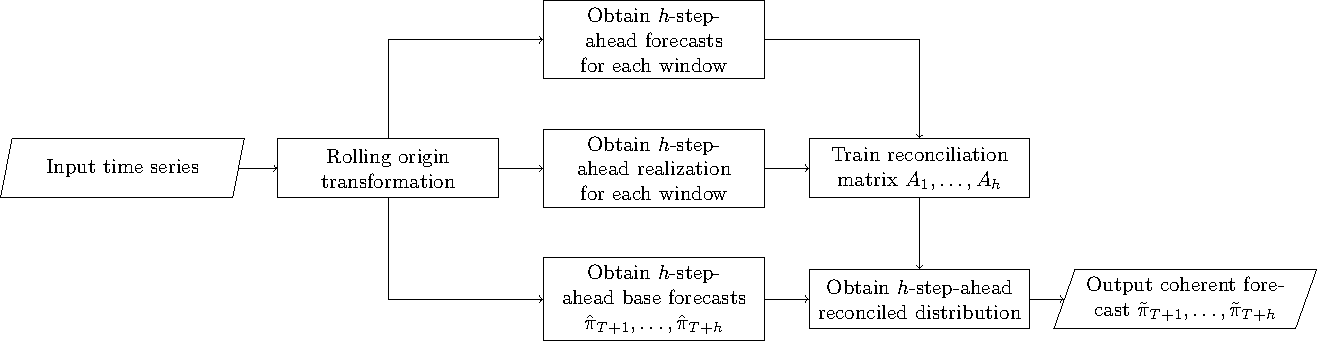
\includegraphics[width=\textwidth]{figures/DFR.pdf}
    \caption{\label{fig:dfr}Flowchart for the DFR algorithm.}
    \end{figure}


    \subsection{Stepwise discrete reconciliation}
    \label{sec:algorithm2}

    Although forcing the parameters of non-nearest points to $0$ reduces the dimension, the exponentially growth of domain cardinalities  still result in an exponentially growth of  number of unknown parameters that need to be estimated.
    As a result, it is impossible to handle high-dimensional hierarchy using the \textbf{DFR} algorithm alone.
    To address this issue, we propose a \textbf{S}tepwise \textbf{D}iscrete \textbf{F}orecast \textbf{R}econciliation (\textbf{SDFR}) algorithm that can overcome the curse of dimensionality.
    Instead of reconciling forecasts of all series at once,  \textbf{SDFR}
    decomposes a high-dimensional hierarchy into multiple two-level hierarchies with three nodes and reconciles these sub-hierarchies step by step using the $\textbf{DFR}$ algorithm shown in \ref{sec:algorithm1}.
    This reduces the number of unknown parameters of each reconciliation process to cubic leve.
    Given some reasonable assumptions, we adjust the reconciled forecasts for these sub-hierarchies to construct joint forecasts for the entire hierarchy.
    Same as \textbf{DFR} algorithm, \textbf{SDFR} also consists of training stage and forecasting stage. The forecasting stage is shown in Algorithm \ref{alg:stepwise}, while training has a similar procedure.
    \begin{algorithm}[ht]
    \caption{\label{alg:stepwise}Stepwise Discrete Forecast Reconciliation (\textbf{SDFR})}
    \SetKwFunction{reconcile}{DFR$_i$}
    \SetKwFunction{bu}{BottomUp}
    \SetKwFunction{adjust}{Adjust}
    \SetKwFunction{construct}{ConstructJointDist}
    \SetKwInOut{Input}{Input}
    \SetKwInOut{Output}{Output}
    \Input{$\hat{\pi}_0,\dots,\hat{\pi}_k$} 
    \For {$i=1,\dots,k-1$}{
      $\hat{\pi}_{\mathbf{S}_{k-i}} \leftarrow$ \bu($\hat\pi_{i+1},\dots,\hat\pi_k$)\;
      \uIf{ i = 1}{
        $\hat{\pi}_{\mathbf{S}_{k-i+1}} \leftarrow \hat\pi_0$ \;
      } 
      \Else{$\hat{\pi}_{\mathbf{S}_{k-i+1}} \leftarrow \sum_{\mathbf{S}_{k-i+2}, y_{i-1}}\tilde{\bpi}(\mathbf{S}_{k-i+2}, y_{i-1}, \mathbf{S}_{k-i+1})$\;
      }
      
      $\tilde{\pi}(\mathbf{S}_{k-i+1}, y_i, \mathbf{S}_{k-i}) \leftarrow$ \reconcile{$\hat{\pi}_{\mathbf{S}_{k-i + 1}}, \hat\pi_{i}, \hat\pi_{\mathbf{S}_{k-i}}$}
    } 
    
    \For {$i=2,\dots,k-1$} {
      $\tilde\pi^{1}_{\mathbf{S}_{k-i+1}} \leftarrow \sum_{\bY_{i-1}}\tilde{\bpi}(\bY_{i-1}, \mathbf{S}_{k-i+1})$ \;
      $\tilde\pi^{2}_{\mathbf{S}_{k-i+1}} \leftarrow \sum_{y_i,\mathbf{S}_{k-1}}\tilde{\bpi}(\mathbf{S}_{k-i+1}, y_i, \mathbf{S}_{k-i})$ \;
      $\tilde\pi'_{\mathbf{S}_{k-1+1}} \leftarrow \frac{1}{2} (\tilde\pi^{1}_{\mathbf{S}_{k-i+1}} + \tilde\pi^{2}_{\mathbf{S}_{k-i+1}}$) \;
      $\tilde{\bpi}'(\bY_{i-1}, \mathbf{S}_{k-i+1}) \leftarrow$ \adjust($\tilde{\bpi}(\bY_{i-1}, \mathbf{S}_{k-i+1}), \tilde{\pi}'_{\mathbf{S}_{k-i+1}})$ \;
      $\tilde{\bpi}'(\mathbf{S}_{k-i+1}, y_i, \mathbf{S}_{k-i}) \leftarrow$ \adjust($\tilde{\bpi}(\mathbf{S}_{k-i+1}, \mathbf{S}_{k-i+1}), y_i, \tilde{\pi}'_{\mathbf{S}_{k-i+1}})$ \;
      $\tilde{\bpi}(\bY_i, \mathbf{S}_{k-i}) \leftarrow$ \construct($\tilde{\bpi}'(\bY_{i-1}, \mathbf{S}_{k-i+1}), \tilde{\bpi}'(\mathbf{S}_{k-i+1}, y_i, \mathbf{S}_{k-i}) $)\; 
    }
    \Output{$\tilde \bpi(\bY_k)$}
    
    \end{algorithm}

  Taking a hierarchy with one total series and $k (k>3)$ bottom series as an example, Algorithm \ref{alg:stepwise} shows how independently generated base forecasts can be reconciled into coherent joint forecasts step-by-step when $k$ is large. 
  Denote the total series as $y_0$ and bottom-level series as $y_1, \dots, y_k$. 
  Denote the vector of first $i+1$ variables as $\mathbf{Y}_i$ and the sum of last $j$ variables as $\mathbf{S}_j$, i.e.
  \[
    \bY_i = (y_0, \dots, y_i)' \quad \mathbf{S}_j = \sum_{l=k-j+1}^{k} y_l.
  \] 
  In general, the hierarchy is split into $k-1$ three-node hierarchies.  
  For each hierarchy $i$, one bottom series (the left node) corresponds to the node $i+1$ in the original hierarchy, i.e., $y_{i}$. The other bottom series (the right node) corresponds to $\mathbf{S}_{k-i}$, which is the sum of the remaining $k-i$ series; thus making $\mathbf{S}_{k-i+1}$ their total node.
  In the training stage, reconciliation model \code{DFR}$_i$ is trained for this hierarchy.
  Base forecasts of the left node are obtained from input, while base forecasts of the right node are obtained using a bottom-up approach that will be discussed in Section~\ref{sec:bottomup}. 
  The base forecasts for the total node are derived from the marginal distribution of that same node from the coherent distribution obtained in the previous step.
  One can obtain base forecasts for the right and total node by forecasting directly $\mathbf{S}_{j}, j=2,\dots,k-1$, which is applicable for cross-sectional hierarchies.
  However in temporal hierarchies, forecasting $\mathbf{S}_{k-i+1}$ means forecasting temporal aggregation of partial time periods, introducingnon-integer frequency problems and making it more challenging to capture time series dynamics.
  Our approach instead offers simple implementation with no extra expert inervation or modelling and can be applied to both cross-sectional and temporal hierarchies. 

  During the forecasting stage, we first pass the base forecasts stepwise into these models to obtain $k-1$ coherent forecasts.
  Adjacent hierarchies share the same node (i.e., $\mathbf{S}_{k-i+1}$), but their marginal forecasts for the shared node (i.e., $\tilde\pi^{2}_{\mathbf{S}_{k-i+1}}$ and $\tilde\pi^{1}_{\mathbf{S}_{k-i+1}}$) are not identical because reconciliation generally changes input forecasts.
  We averages these two marginal forecasts and pass their average into the \code{Adjust} algorithm, which adjusts the joint distributions from two adjacent steps to make their marginalisations of the shared node equivalent to the average.
  The two adjusted distributions are then passed into the \code{ConstructJointDist} algorithm to construct a new joint distribution.
  For space-saving purpose here, the \code{Adjust} and \code{ConstructJointDist} algorithms are shown in \ref{appendix:adjust}.

  Note that in our proposed algorithm, the order of the bottom-level series does not matter.
  One can involve forecast model combination technique by averaging multiple results from randomly reordering the bottom-level series; this reduces forecast uncertainty introduced by the \code{Adjust} and \code{ConstructJointDist} algorithms.
  When handling hierarchy with more aggregation levels, we can repeat above procedure for each aggregated series either in a bottom-up or top-down manner. This means we reconcile the base forecasts of one level and use the reconciled forecasts as base children forecasts(bottom-up) or base parent forecasts (top-down) to reconcile next level.

  

    \subsection{Probabilistic extensions of bottom-up and top-down methods for count series}

    The top-down and bottom-up methods are traditional and straightforward techniques used for hierarchical point forecasting. 
    These methods requires forecasts at a single level, which they then use to generate forecasts at other levels through disaggregation (top-down) or aggregation (bottom-up).
    In this section, we extend this idea to discrete cases by introducing the Discrete Bottom-Up (DBU) and Discrete Top-Down (DTD) methods. These approaches can produce distributional forecasts for count time series based on base forecasts from a single level.
    We also show how these two approaches can be incorporated into the proposed linear reconciliation method.

    \subsubsection*{\textbf{Discrete bottom-up}}
    \label{sec:bottomup}

    The discrete bottom-up method constructs a coherent distribution by assuming independent bottom-level forecasts.
    This method follows the same procedure as constructing base forecasts explained in Section~\ref{sec:algorithm1} except that the base forecasts of aggregated series are excluded.
    Using the three-variables example, $\tilde{\pi}_{(000)} = Pr(Y_1=0)\times Pr(Y_2=0)$. 
    The linear reconciliation framework can also incorporate this method by marginalising out all aggregated time series from the incoherent base distribution, which yields \[
    \mathbf{A} = [\mathbf{I}_4\quad \mathbf{I}_4 \quad \mathbf{I}_4 ],
    \]
    Note that the mean point forecasts obtained from this coherent distributionl's marginal distribution of  are identical to the those obtained by directly aggregating mean forecasts of bottom-level series.
    In other words, discrete bottom-up is compatible with the traditional bottom-up methods.

    Although it is possible to learn dependence structure between bottom-level time series (e.g., empirical copulas used in \citealp{bentaiebHierarchicalProbabilisticForecasting2020}), we stick to the independence assumption due to its simplicity.

    \subsubsection*{\textbf{Discrete top-down}}

    The discrete top-down method extends the traditional top-down by proportionally disaggregating the probabilities of each point of the total series into all possible coherent points, using a ratio computed from historical occurrences.
    For example, if there are $40$ $(0, 1, 1)$ points and $60$ $(1, 0, 1) $ points observed in the three-variables scenario where $Pr(y_3) = 0.4$, the probabilities of possible coherent points would be calculated as follows: $\tilde \pi_{(011)} = 0.4\times 0.4$ and $\tilde \pi_{(101)} = 0.4\times 0.6$.
    This method can also be considered as a special case of Equation (\ref{eq:framework}), where
    \[
    \mathbf{A} = \left[\begin{matrix}
      1 & 1 & 1 & 1 & 0 & 0 & 0 & 0 & 0 & 0 & 0 & 0 \\
      0 & 0 & 0 & 0 & 0.4 & 0.4 & 0.4 & 0.4 & 0 & 0 & 0 & 0 \\      
      0 & 0 & 0 & 0 & 0.6 & 0.6 & 0.6 & 0.6 & 0 & 0 & 0 & 0 \\
      0 & 0 & 0 & 0 & 0 & 0 & 0 & 0 & 1 & 1 & 1 & 1  
    \end{matrix}\right].
    \]

\section{Simulation}
\label{sec:simulation}

To showcase the effectiveness of our proposed framework, we conduct two simulation experiments in distinct contexts: one for cross-sectional settings and another for temporal settings. 
     
  \subsection{Cross-sectional hierarchy}
  \label{sec:cross-sectional_simu}
    \subsubsection{Simulation setup}
    This subsection considers the three-variables hierarchy depicted in Section~\ref{sec:example}.
    The binary count time series at the bottom level are generated based on underlying latent variables. 
    We assume that these variables follow a bivariate VAR(1) process
    \[\mathbf{s}_t = \mathbf{\Phi}\mathbf{s}_{t-1}+\boldsymbol{\eta}_t,\]
    where
    \[
      \mathbf{\Phi} = \left[\begin{matrix}
        \alpha & 0 \\
        0 & \beta
      \end{matrix}\right], \boldsymbol{\eta} \sim \mathcal{N}\left(\mathbf{0}, \left[\begin{matrix}
        0.1 & 0.05 \\
        0.05 & 0.1 
      \end{matrix}\right]\right), \mathbf{s}_{-1} = \left[
        \begin{matrix}0 \\ 0\end{matrix}
      \right].
    \]
    $\alpha$ and $\beta$ are uniformly generated from $[0.4, 0.5]$ and $[0.3,0.5]$, respectively. 
    This ensures the stability of the generated time series.
    The error term $\boldsymbol{\eta}$ implies positive correlation between the two series and ensures reasonable range of the latent state.
    Observations are transformed from the state series using a sign function:
    \[
        Y_i = \mathbb{I}(\sigma(s_i) > 0.5), i\in\{1, 2\},\quad \sigma(s) = \frac{\exp(s)}{1+\exp(s)}.
    \]

    We produce and evaluate one-step-ahead forecasts in this experiment.
    For each binary series, we generate $480$ observations; the rolling origin strategy with $150$ observations used to train the base forecasting models is employed, yielding $330$ samples.
    The first $300$ samples are used to train the \textbf{DFR} model, while remaining $30$ samples are used to test performance.
    
    The base probabilistic forecasts are obtained independently using the binomial AR(1) model(\citealp{weissParameterEstimationBinomial2013}), which is suitable for count time series with a finite range.
    We evaluate the performance based on average brier scores of the joint distribution of hierarchy and marginal distribution of each series on the $30$ testing samples.
     
    \subsubsection{Simulation results}
    The above procedure was repeated $1000$ times. 
    Table~\ref{tab:sim_crosssectional_res_dist} summarizes the average Brier Scores of the $1000$ samples, compared with base forecasts, discrete bottom-up and discret top-down method.
    The best average performance out of the four approaches is indicated by bold text in each row.
    DFR performs the best for both the single series and the hierarchy. 
    The discrete bottom-up method beats discrete top-down in both the total and bottom levels, indicating the inferiority of the base forecasts of the total series.
    However, DFR shows considerable improvement in the accuracy of the total series, which implies its ability to mitigate the risk of model misspecification.
    Similar results were obtained from forecast reconciliation for continuous variables as well.
    Note that the Brier Score for the joint distribution of the base method is significantly larger than that of other methods, primarily because of to its incoherency nature.
    
    We also performed the MCB tests (\citealp{koningM3CompetitionStatistical2005}) at a 95\% level of confidence to test the statistical significance of differences in accuracy between these approaches. 
    This testing approach computes the mean ranks of the four approaches across whole simulation set without imposing any distributional assumptions.
    Non-overlapping grey intervals indicate statistically significant differences between methods.
    As shown in Figure~\ref{fig:sim_temporal_mcb_prob}, DFR performs more significantly than all other approaches.
    Please note that MCB tests for bottom series are conducted on all samples at the bottom level.
  
    \begin{figure}
      \centering
      \label{fig:mcb_crosssectional}
      \caption{Average ranks and 95\% confidence intervals for the four approaches in the cross-sectional simulation. The overall ranks of the approaches in terms of Brier scores are shown to the left of their names.}
      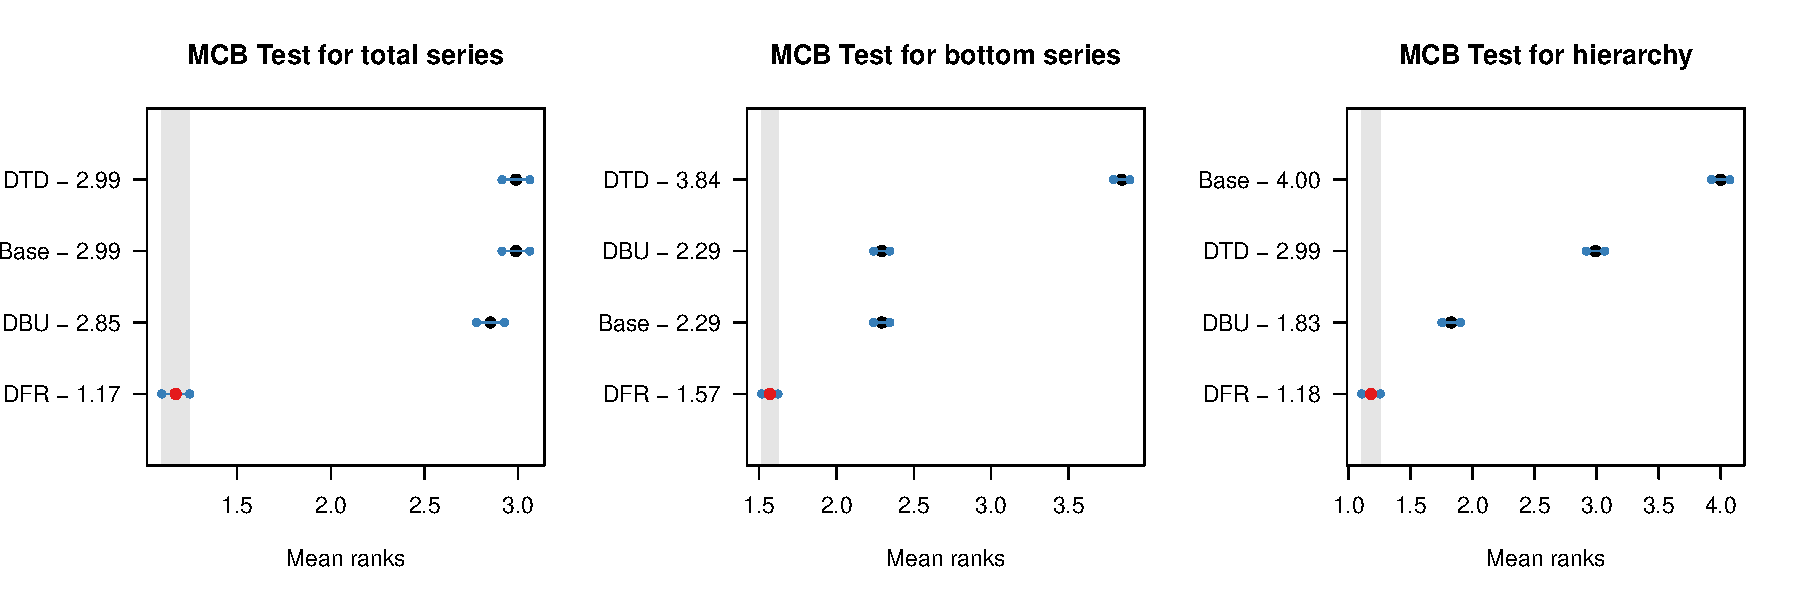
\includegraphics[width=\textwidth]{figures/cross_sectional_mcb.pdf}
    \end{figure}
    
    
    \begin{table}
      \centering
      \caption{\label{tab:sim_crosssectional_res_dist} Probabilistic forecast performance summary of cross-sectional setting.}
      \begin{tabular}{lcccc}
      \toprule
      \multicolumn{5}{c}{Brier Score ($\times 10^{-2}$)}\\ 
      & Base & Bottom-Up & Top-Down & DFR \\\midrule
      $Y_1$ & 25.4 & 25.4 & 34.9 & \textbf{24.4} \\
      $Y_2$ & 27.8 & 27.8 & 34.8 & \textbf{25.7}\\
      $Y_3$ & 49.7 & 49.5 & 49.7 & \textbf{42.0} \\
      $\bY$ & 74.4 & 47.8 & 56.1 & \textbf{44.0} \\
      \bottomrule
      \end{tabular} 
    \end{table}
     
     
     \subsection{Temporal hierarchy}

     We now consider a daily temporal scenario consisting of one total series and $7$ bottom-level series. 
     This type of setting is frequently encountered in supply chain management, where daily and weekly forecasts are required to support operational decisions (\citealp{syntetosSupplyChainForecasting2016}).
     The bottom-level time series are restricted to values of 0 or 1.
     Despite this limitation, the hierarchy's domain remains extensive, making it difficult to estimate a complete reconciliation matrix with limited observations in practice. 
     Therefore, we employ the stepwise reconciliation algorithm outlined in Section \ref{sec:algorithm2}. 
     
     \subsubsection{Simulation setup}
     
     While intermittent series are characterized by fluctuating demand intervals and size at lower levels, they may exhibit seasonality and trend when temporally aggregated into higher levels (\Citealp{kourentzesElucidateStructureIntermittent2021}).
     Based on this understanding, we initially simulate weekly time series with a seasonal period of $4$, which are subsequently disaggregated into daily time series.
     
     Assuming that the weekly time series follow a Poisson distribution, we first simulate the conditional mean series utilising the autoregressive integrated moving average(ARIMA)  process. This procedure is implemented with the \code{gratis} package for \proglang{R} programming language. 
     The controlled parameters are shown in Table~\ref{tab:parameters}. Additional parameters are randomly produced by the package to ensure the diversity of the simulated series (\Citealp{kangGRATISGeneRAtingTIme2020}). 
     Given that the domain of the weekly time series in our context is finite (i.e., $\leq 7$), we linearly map the generated conditional mean series into the range of $[2.5, 4.5]$. 
     Subsequently, we simulate the Poisson distributed series based on the conditional mean series. Values exceeding $7$ are set to $7$.
     
     \begin{table}[h]
       \centering
       \caption{\label{tab:parameters} Selected parameters of the ARIMA process used to simulate the conditional mean of weekly time series in the temporal setting.}
       \begin{tabular}{lc}
         \toprule
         Parameter name & Value \\ \midrule
         Frequency & 4 \\
         Number of autoregressive terms & 3 \\
         Difference order & 0 \\
         Seasonal difference order & 0 \\ \bottomrule
       \end{tabular}
     \end{table}
     
     The weekly time series are then disaggregated into daily time series by randomly selecting days for which $Y=1$ and maintaining coherence. 
     We first simulate seven probabilities based on seven independent Beta distributions $\textrm{B}(\alpha, \beta)$, corresponding to probabilities of $Y=1$ from Monday to Sunday. 
     The values of the $w$ days with the highest probabilities are set to $1$, while others are set to $0$. Here, $w$ denotes the value of the corresponding weekly observation.
     $\beta$ is set to $4$ and $\alpha$ is set to $\alpha_i = i i=1,\dots,7$, allowing for the probabilities of $Y=1$ to increase gradually from $i=1$ to $i=7$, suggesting potential seasonality.
     
     For each daily time series, $1003$ observations are generated, and the initial $100$ observations are discarded as warm-ups. Analogous to Section~\ref{sec:cross-sectional_simu}, we utilise the rolling origin strategy with a fixed look-back window size of $350$, yielding $547$ windows.
     For each rolling timestamp, the most recent $350$ observations are used as input to generate probabilistic forecasts for the following seven days. 
     The initial $526$ samples are used to train the reconciliation model, and the final $21$ samples were are to assess the forecasting performance.
     
     Base forecasts of daily time series are generated utilising an autoregressive logistic model. 
     Specifically, for each origin, we construct an individual logistic model that employs the previous six observations and weekly dummy variables as regressors to predict the subsequent observation. 
     To generate forecasts for the final seven days, at each step, we use the predicted value from the previous step as a regressor to predict the next step recursively. 
     We implement the logistic regression model with the \code{glm} function in \proglang{R} programming language.
     
     Base forecasts of weekly time series are generated using integer-valued GARCH $(\textrm{INGARCH})$ models (\Citealp{fokianosPoissonAutoregression2009}). 
     Assuming that observations are Poisson distributed, the $\textrm{INGARCH}$ model utilises past observations and conditional mean to fit the conditional mean of current observation.
     For the sake of simplicity, we construct $\textrm{INGARCH}(3, 3)$ models for all weekly time series, which takes the conditional mean and observations from the most recent three steps as regressors. 
     We implement the $\textrm{INGARCH}$ model using the \code{tscount} package(\Citealp{liboschikTscountPackageAnalysis2017}) for \proglang{R}.
     Given the predicted mean of Poisson distribution within the forecast horizon, we add the probability of the series taking values greater than its maximum up to the probability of taking its maximum value.
     The base forecasts are then reconciled using the \textrm{SDFR} algorithm.

     
     \subsubsection{Simulation results}
     We repeated the simulation pr ocess $1000$ times.
     Table~\ref{tab:sim_temporal_res_dist} summarizes the probabilistic forecast performance of the stepwise reconciliation model, in comparison to base forecasts, discree bottom-up and discrete top-down method.
     $Y_1,\dots,Y_7$ represent the daily series at the bottom level, while $Y_8$ denotes the weekly series at the total level.
     Although SDFR does not enhance forecast accuracies for all series, the results
     demonstrate a compromise between discrete top-down and discrete bottom-up methods. 
     One intriguing observation is that the forecasting accuracy improves for $Y_4$ through $Y_7$. 
     This could be attributed to the stepwise implementation of SDFR, which progresses from $Y_1$ to $Y_7$. The coherent forecasts of previous series must be adjusted multiple times to construct the final joint distribution, thereby introducing uncertainty.
     Another explanation could be the effective utilisation of forecast combination, where the bottom-level series corresponding to the end of the week incorporate more forecasts than preceding ones.
     Surprisingly, the forecast accuracy of the total series does not exhibit significant deviation from base forecasts,  even though it is adjusted most frequently, showcasing the robustness of \textbf{SDFR}.
     It is crucial to note that the results could vary if the SDFR algorithm is implemented in a different step order.
     Additionally, the performance could be enhanced if we average multiple reconciled forecasts from various orderings.
     Figure~\ref{fig:sim_temporal_mcb_prob} displays the results of MCB tests of differences in forecast performance. The outcomes lead to similar conclusions to those derived from Table~\ref{tab:sim_temporal_res_dist}. 
     
     \begin{table}
     \centering
     \caption{\label{tab:sim_temporal_res_dist} Probabilistic forecast performance summary of temporal setting.}
     \begin{tabular}{lcccc}
     \toprule
     \multicolumn{5}{c}{Brier Score ($\times 10^{-3}$)}\\ 
      & Base & Bottom-Up & Top-Down & SDFR \\\midrule
     $Y_1$ & \textbf{408.2} & \textbf{408.2} & 494.1 & 409.9 \\
     $Y_2$ & \textbf{414.3} & \textbf{414.3} & 496.1 & 415.8\\
     $Y_3$ & \textbf{420.9} & \textbf{420.9} & 498.6 & 421.0\\
     $Y_4$ & 430.3 & 430.3  & 500.4          & \textbf{427.9}\\
     $Y_5$ & 435.5 & 435.5  & 502.2          & \textbf{430.9} \\
     $Y_6$ & 440.0 & 440.0  & 502.6          & \textbf{433.2} \\
     $Y_7$ & 443.0 & 443.0  & 502.9          & \textbf{438.9} \\
     $Y_8$ & \textbf{825.8} & 834.5          & \textbf{825.8} & 831.0\\
     $\bY$ & 995.4 & 977.8  & 993.6          & \textbf{977.4} \\
     \bottomrule
     \end{tabular}
     \end{table}
     
     
     \begin{figure}
       \caption{\label{fig:sim_temporal_mcb_prob}Average ranks and 95\% confidence intervals for the four approaches in the temporal simulation. The overall ranks of the approaches in terms of brier scores are shown to the left of their names.}
       \subfloat{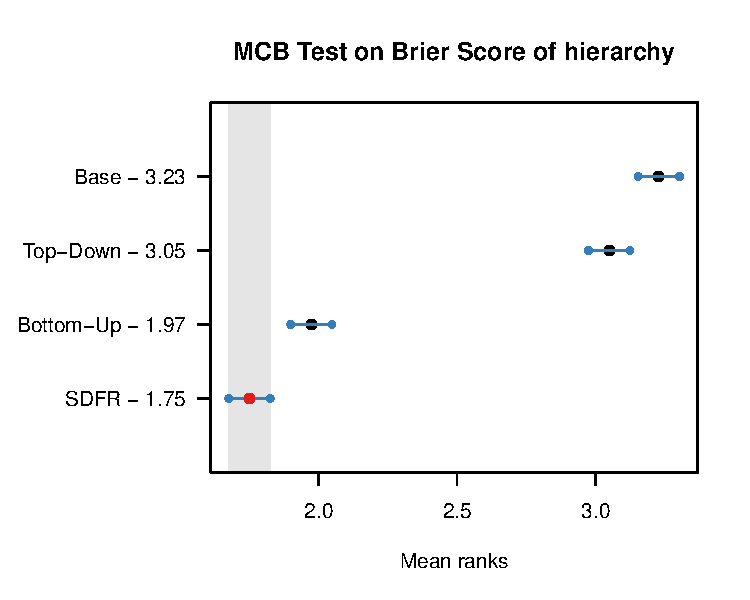
\includegraphics[width=0.31\textwidth]{figures/temporal_mcb_BS_hierarchy.pdf}} \qquad
       \subfloat{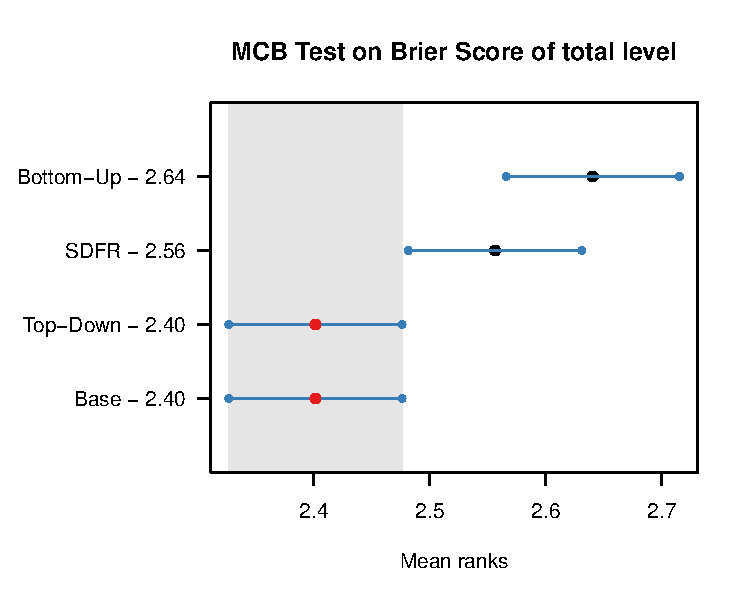
\includegraphics[width=0.31\textwidth]{figures/temporal_mcb_BS_total.pdf}} \qquad
       \subfloat{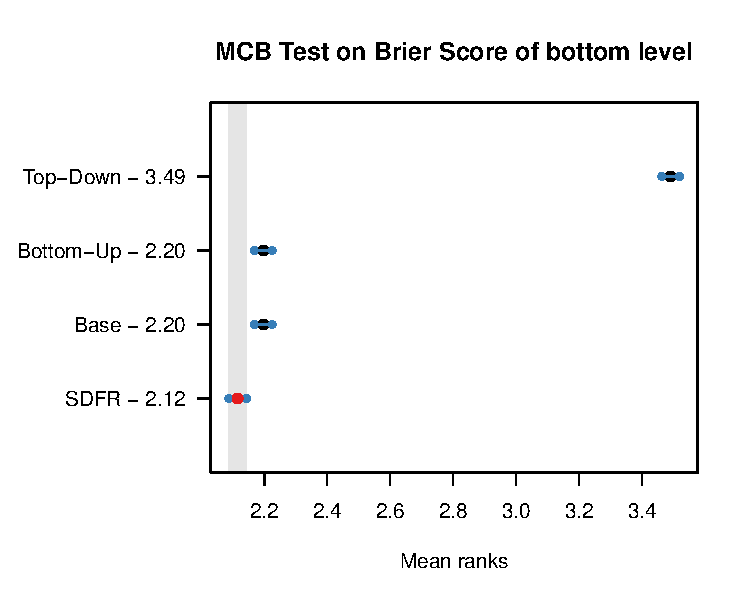
\includegraphics[width=0.31\textwidth]{figures/temporal_mcb_BS_bottom.pdf}}
     \end{figure}     

     \section{Empirical study}
     \label{sec:application}
     In this section, we utilize the proposed DFR algorithm to analyse two publicly available real-world datasets.
     Section~\ref{sec:application_crime} concentrates on temporal hierarchy and forecasts the number of criminal offences in Washington D.C. 
     Meanwhile, Section~\ref{sec:application_mortality} constructs and forecasts cross-sectional count hierarchical time series based on mortality thresholds. 
     
     \subsection{Application: forecasting crime in Washington D.C.}
     \label{sec:application_crime}
     
     Forecasting crime numbers in a specific area is vital for managing public health and police resource.
     However, forecasting becomes more challenging when dealing with smaller areas where crime numbers are sparse.
     In this subsection, we apply our DFR algorithm to predict the number of offence crimes in census tracts located in Washington, D.C. 
     The original dataset\footnote{The dataset can be downloaded from \url{https://crimecards.dc.gov/}.} contains all reported crimes from 2014 to 2022 in Washington D.C., which have been aggregated into weekly time series according to location and crime type. 
     Considering the domain of the number of crimes, we perform experiments on all time series whose location type is a census tract and crime type is offence.
     As a result, we obtain $231$ weekly time series; each representing the number of offence crimes committed within one census tract.
     
     The crime numbers time series are potentially autocorrelated (\citealp{aldor-noimanSpatioTemporalLowCount2013}). 
     Our objective is to generate coherent probabilistic forecasts for the next four weeks.
     To achieve this, we construct two-level temporal hierarchies that consists of weekly(bottom level) and four-weekly(total level) frequencies and develop an individual DFR model for each time series.
     Additionally, we restrict the maximum value (i.e., domain of bottom level in the \textbf{DFR} model) of the weekly time series as follows: if the largest observation is $1$, then its domain is set to $[0, 1]$. 
     Otherwise, it is set to $[0, 1, 2]$. 
     Any observation exceeding $2$ is truncated at $2$. 
     It should be noted that less than one percent of observations surpass $2$, so these adjustments have a negligible impact on our final results.
     
     We adopt the rolling origin strategy to train and evaluate our discrete reconciliation model. 
     Initially, we produce four-step-ahead probabilistic forecasts using INGARCH(3, 4) from a time series of $53$ weeks. 
     Subsequently, we augment the training data by one week and produce new probabilistic forecasts. 
     At each step, to obtain the probabilistic forecasts for the total leve, we first aggregate the weekly series into four-weekly time series and then use INGARCH(2, 2) to produce one-step-ahead forecasts.
     We only use windows with forecast horizons starting before $2022$ as training samples; all remaining windows are used for performance evaluation purposes.
     We repeat the above procedure for every census tract, resulting in a total of $3696$ samples ($231$ census tracts multiplied by $16$ test samples per census tract). 
     These reconciled forecasts are then used to evaluate forecasting performance. 
     
     We calculate Brier Scores for each sample at the total level, the bottom level and entire hierarchy. 
     Table~\ref{tab:crime_bs} summarises the mean and median negative Brier Score of the $3696$ samples.
     We also perform the MCB Test to indicate the significance of the difference, with results shown in Figure~\ref{fig:application_crime}.
     
     \begin{table}[h]
       \centering
       \caption{\label{tab:crime_bs}Summarised negative Brier Score($\times 10^{-2}$) of test samples in crime forecasting application.}
       \begin{tabular}{ccccccccc}
       \toprule
       &\multicolumn{4}{c}{Mean} 
       & \multicolumn{4}{c}{Median} \\ \cmidrule(lr){2-5} \cmidrule(lr){6-9}
        & Base & Bottom-Up & Top-Down & DFR &  Base & Bottom-Up & Top-Down & DFR \\\midrule
       Total & 58.47 & \textbf{58.07} & 58.47 & 58.12 & 66.64 & 65.28 & 66.64 & \textbf{64.75} \\
       Bottom & 34.41 & 34.41 & 34.80 & \textbf{34.30} & 13.73 & 13.73 & 13.28 & \textbf{10.82}\\
       Hierarchy & 73.87 & \textbf{67.87} & 68.33 & 67.97 & 97.66 & 92.70 & 93.08 & \textbf{92.42}\\
       \bottomrule
       \end{tabular}
       \end{table}
     
     \begin{figure}[h]
       \caption{\label{fig:application_crime}Average ranks and 95\% confidence intervals for the four approaches in the crime forecasting application. The overall ranks of the approaches in terms of brier scores are shown to the left of their names.}
       \centering
       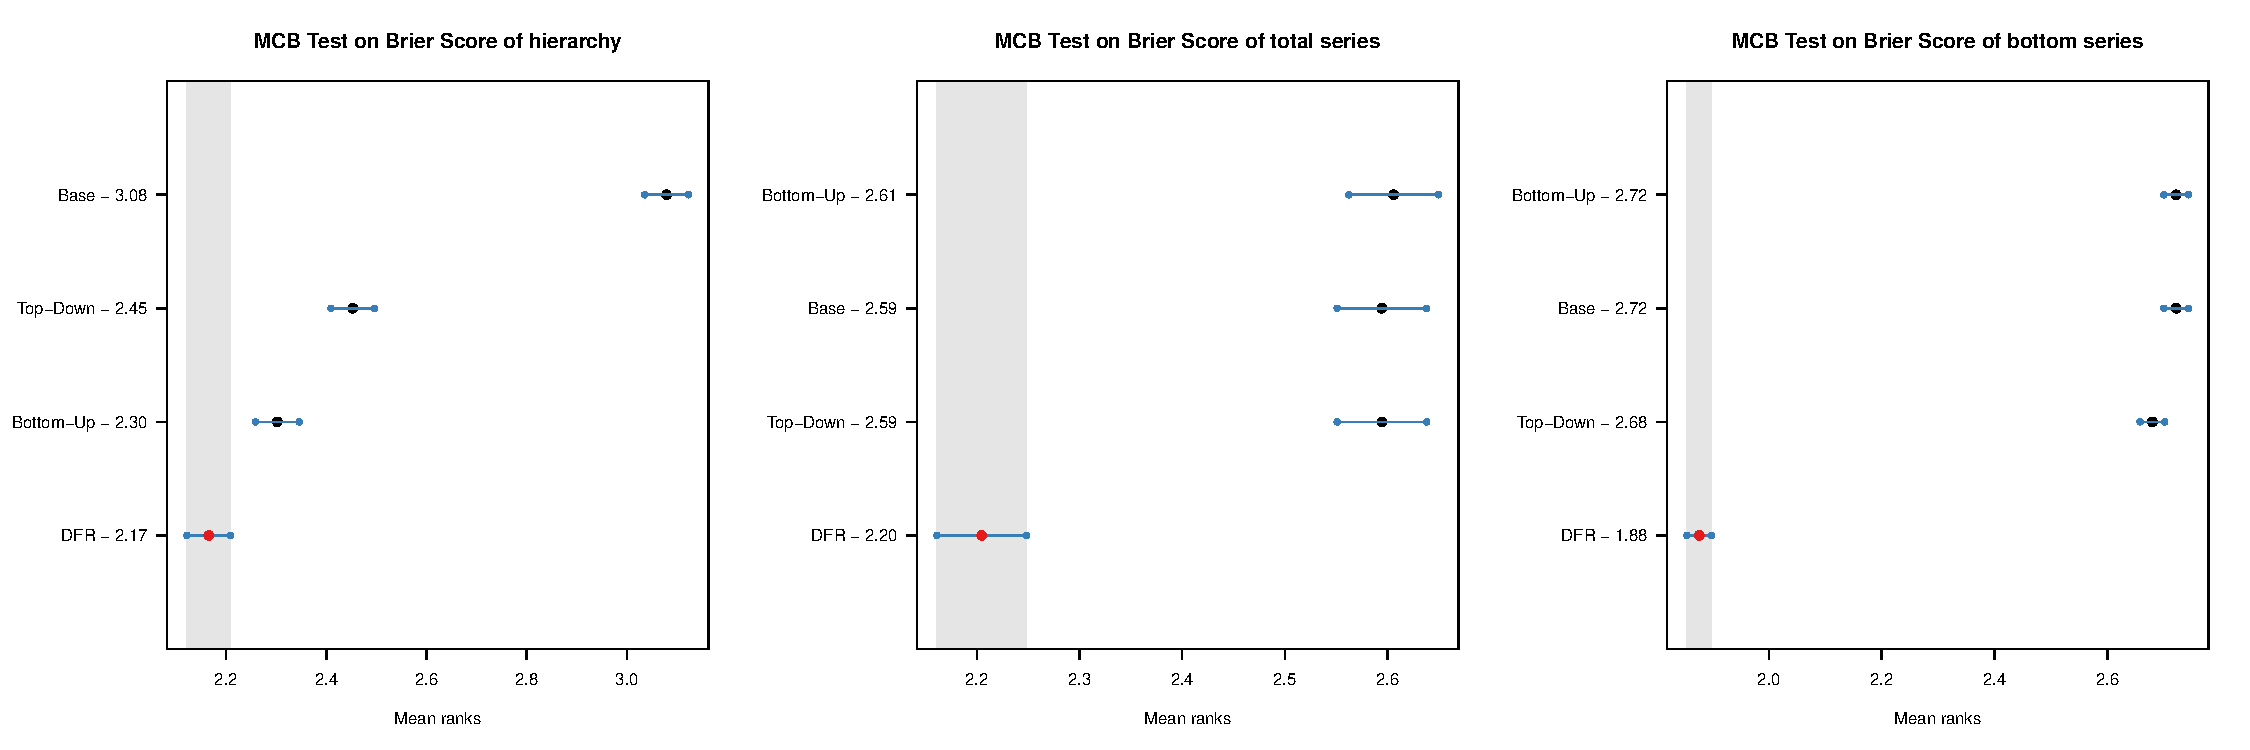
\includegraphics[width=\textwidth]{figures/dc_crime_bs.pdf}
     \end{figure}
     
     
     In Table~\ref{tab:crime_bs}, the left panel shows that DFR algorithm outperforms base forecasts for all levels in terms of mean Brier Scores. This indicates that DFR not only produces coherent forecasts but also improves forecasting accuracy.
     The discrete bottom-up performs better than other methods, including the discrete top-down method, which suggests inferiority in total-level forecasts. 
     Although on average, the right panel shows that discrete bottom-up performs slightly better than DFR for both total level and whole hierarchy, DFR outperforms all other approaches in terms of median brier scores.
     The most significant improvement occurs at the bottom level.
     The MCB test plots in Figure~\ref{fig:application_crime} demonstrate a statistical difference between DFR and other methods.
     Furthermore, results from testc conducted on all bottom-level series support the conclusion drawn from the right panel of Table~\ref{tab:crime_bs}.
     These findings imply that DFR is more effective than other approaches for more HTSs. 
     
     \subsection{Application: forecasting mortality threshold exceedance in Australia}
     \label{sec:application_mortality}
     The high mortality rate among the population is a major concern for practitioners. 
     They are particularly worried about risks that arise when mortality exceeds a certain threshold. 
     One example of this is the Vita Capital mortality catastrophe bonds, which provide coverage for excess mortality risks in various areas. 
     If the mortality rate in one or more areas surpasses specific thresholds, investors may not receive their principal payments from the issuer.
     In these situations, joint probabilistic forecasts become essential as they offer a comprehensive view of potential future outcomes. 
     These forecasts are especially critical when there is dependence between mortalities in target areas.
     
     We conduct an experiment using yearly mortality data collected from 1921 to 2020 in Australia.
     The data is grouped by age, and we focus on the mortality of elder groups: $[55, 64]$, $[65, 74]$, $[75, 84]$, $[85, )$. 
     We construct a two-level hierarchy, where the bottom level includes 
     $4$ binary series that indicates whether the mortality of each corresponding age group exceeds a given threshold for that year.
     We then aggregate these bottom-level series to obtain a total series indicating how many groups exceed their thresholds.
     
     There are no ready-to-use thresholds available for specific age groups and years. 
     To address this, we establish a custom rule for illustrative purposes in this experiment. 
     We assume that mortality decreases linearly over a short period (e.g., ten years) due to the advancements in technology, economy, medical conditions and other factors. 
     Using this assumption, we determine the ``expected'' threshold for a particular age group in a specific year by applying the following formula:
     \[
       \text{threshold}_t = 1.005 \times (m_t - (m_{t-11} - m_{t-1})/10),
     \]
     where $m_t$ represents the mortality at year $t$, and $1.005$ is an excess death coefficient manually specified by us.
     We then transform the mortality series into binary series by comparing actual mortality rates to the ``expected'' thresholds.
     
     In this experiment, we also employ the rolling origin strategy with a starting window size of $20$, resulting in $69$ samples.
     The first $59$ of them are utilised to train the DFR model, while the remaining samples are used to test forecast performances.
     INGARCH(3, 5) models generated base forecasts for all series. 
     
     Brier Scores are evaluated for each age group, the total series and the entrie hierarchy.
     Table~\ref{tab:mortality_age} presents an overview of the average negative Brier Scores across the ten testing samples.
     The DFR approach yields the most accurate joint forecasts for the hierarchy and outperforms other methods for most single series as well.
     It is disappointing to note that the performance of the oldest group (i.e. $[85, )$) decreases, given that this group is typically a priority in practice.
     However, this phenomenon also occurs with reconciliation frameworks in continuous cases. 
     Although such frameworks generally improve forecast accuracy across all series, some individual series may experience decreased accuracy (\citealp{zhangOptimalReconciliationImmutable2022a}).
     
     
     \begin{table}
       \centering
       \caption{\label{tab:mortality_age} Probabilistic forecast performance summary of mortality application.}
       \begin{tabular}{lcccc}
       \toprule
       \multicolumn{5}{c}{Brier Score ($\times 10^{-3}$)}\\ 
       & Base & Bottom-Up & Top-Down & DFR \\\midrule
       Total & 638.0 & 626.7 & 638.0 & \textbf{590.8} \\
       $[55, 64]$ & \textbf{174.5} & \textbf{174.5} & 203.3 & 175.1 \\
       $[65, 74]$ & 138.3 & 138.3 & 142.9 & \textbf{128.9}\\
       $[75, 84]$ & 205.5 & 205.5 & 324.4 & \textbf{160.4}\\
       $[85, )$ & 495.3 & 495.3 & \textbf{444.2} & 521.6\\
       Hierarchy & 882.4 & 697.0 & 736.7 & \textbf{675.2} \\
       \bottomrule
      \end{tabular}
     \end{table}

     \section{Discussion}

    

     Distributional forecasts are becoming increasingly important in both academic and industry settings for operational research. In the context of hierarchical forecasting, \cite{kolassaWeWantCoherent2022} suggests shifting focus from coherent point forecasts to coherent probabilistic forecasts. 
     The proposed discrete reconciliation framework can generate coherent distributional forecasts for discrete-valued HTSs.  
     Summary statistics such as median, mean, and quantiles can be derived from the marginal distribution obtained from the distributional forecasts. 
     It is worth noting that mean point forecasts obtained through this way are also coherent in terms of aggregation.
     Moreover, our methods offer precise distribution instead of relying on empirical distribution derived from sampling as seen in previous studies (e.g., \citealp{jeonProbabilisticForecastReconciliation2019,coraniProbabilisticReconciliationCount2022}).

     This paper focuses on linear reconciliation, achieved by multiplying the base incoherent probability vector with a reconciliation matrix. 
     From a machine learning perspective, this procedure can be viewed as a classification problem with $r$ categories and a $q$-dimensional input. Machine learning models such as specifically designed neural networks can be utilized to solve this problem. 
     In the scenario where thousands of time series need to forecast, cross-learning techniques can be employed to construct a global non-linear reconciliation model. 

     One area for improvement of the proposed DFR algorithm is that it can not be easily applied to a large hierarchy which requires more observations and computational resources due to the curse of dimensionality.
     While the SDFR algorithm mitigates this problem, it also introduces additional uncertainty. 
     We suggest applying the proposed algorithm to a small hierarchy with finite domains. 
     When applying to large hierarchies, the bottom-level series should be low-count, such as binary.

     In our experiments, we have observed that the accuracy of some series' base forecasts is not ideal. 
     We attribute this to three reasons. Firstly, it is challenging to forecast low count time series with excess zeros accurately. 
     Secondly, we have not used state-of-the-art forecasting methods for such time series as proposed by \cite{berryBayesianForecastingMany2020a} and \cite{weiEmpiricalLikelihoodRatio2021}. 
     Thirdly, the parameters of the employed models are not carefully selected. 
     To improve performance in future work, we suggest using more modern forecasting methods and carefully selecting both models and parameters.

     This paper presents two simulation experiments and two empirical studies.
     While the experiment results show a significant improvement in accuracy, the applications are not entirely natural. 
     For instance, in the crime forecasting experiment where extreme values are usually crucial, we truncate the infinite domain of crime numbers. 
     In the mortality experiment, binary series are created based on custom thresholds.
     Future research could apply our proposed frameworks to real scenarios where time series have finite domains and deterministic constraints exist between them.  
     It is important to note that  these constraints may not only be based on aggregation, but can also be other deterministic function such as logical operators.


     

     \section{Conclusion}
     \label{sec:conclusion}
     
     This paper develops a novel forecast reconciliation framework for count hierarchical time series. 
     The framework involves assigning probabilities from incoherent points to coherent points, similar to the mapping approach used for continuous time series.
     We further propose a linear reconciliation algorithm that minimises the penalized brier score of reconciled probabilistic forecasts.
     To address the exponential growth of the domain, we introduce a stepwise discrete reconciliation algorithm by breaking down a large hierarchy into smaller ones.
     We also propose probabilistic extensions of traditional top-down and bottom-up methods for count time series.
     
     Our DFR and SDFR algorithms produce coherent probabilistic forecasts and improve forecast accuracy. 
     We demonstrate this through simulation experiments on cross-sectional and temporal hierarchies, where our algorithms outperform discrete top-down and discrete bottom-up approaches. Additionally, we apply the DFR algorithm to forecast crime numbers in Washington D.C. and mortality threshold exceedance of elder groups in Australia with promising results.
     The results indicate the potential of the proposed algorithms to be applied in reality.
     
     One key factor contributing to our strong results is  the utilization of forecast combinations.
     Similar to reconciliation approaches for continuous variables, our framework combines forecasts and the information used to produce forecasts at different levels.
     Also of importance is that our models train the reconciliation weights using out-of-sample forecasts generated by the rolling origin strategy, leading to robust results. 
     
     
     While this work provides an explanatory attempt at discrete hierarchical time series forecasting, future research should focus more on real-world management problems associated with discrete cases. Count hierarchical time series forecasting remains an open issue that requires further attention from researchers in this area.


\newpage

\appendix

\section{Algorithms}
\label{appendix:adjust}

The \code{Adjust} algorithm is used to adjust an existing multivariate joint distribution to make its marginalisation over one of the variables equal to that given by a reconciled distribution is a single step of the stepwise procedure.

\begin{algorithm}[H]
  \label{alg:adjust}
  \caption{Adjust}
  \SetKwInOut{Input}{Input}
  \SetKwInOut{Output}{Output}
  \Input{$\bpi(y_0,y_1,\dots,y_i), \tilde\pi_i, y_i \in \{0,1,\dots,k_i\}$}

  $\bpi(y_0,\dots,y_{i-1}) = \sum_{y_i}\bpi(y_0,\dots,y_i)$\;
  $\pi_i = \sum_{y_0,\dots,y_{i-1}}\bpi(y_0,\dots,y_i)$ \;
  \For { $j = 0,\dots,k_i$} {
    $\bpi'(y_0,\dots,y_{i-1}, y_i=j) = \bpi(y_0,\dots,y_{i-1}) \times \frac{\tilde\pi_i}{\pi_i}$ \;
  }

  \Output{$\bpi'(y_0,\dots,y_i)$}
  
 \end{algorithm}


 The \code{ConstructJointDist} algorithm constructs a new joint construct given two joint distributions. 
 Consider variables $y_1, \bY_2, y_3, y_4, \bY_5$, where $\bY_2$ and $\bY_5$ are vectors and $y_1, y_3, y_4$ are scalars. 
 They have the following relations
 \[
  y_1 = |\bY_2|_1 + y_3, \quad y_3 = y_4 + |\bY_5|_1,
 \]
 where $|\cdot|_1$ represents the sum of all the variables in the vector.
 The given distributions are $\bpi(y_1, \bY_2, y_3)$ and $\bpi(y_3, y_4, \bY_5)$.
 The marginal distributions of $y_3$ derived from the two distributions are the same, i.e.,
 \[
  \sum_{y_3} \bpi(y_1, \bY_2, y_3) = \sum_{y_3}\bpi(y_3, y_4, \bY_5)
\]
 Assuming the joint distribution of $y_1$ and $\bY_2$ is independent of the joint distribution of $y_4$ and $\bY_5$ given $y_3$, we can obtain the probability of one point in the new joint distribution using the following equation: \[
   \begin{aligned}
  &\text{Pr}(y_1=a_1,\bY_2=\mathbf{a}_2, y_4=a_4, \bY_5 = \mathbf{a}_5) =\\ &\text{Pr} (y_1=a_1,\bY_2=\mathbf{a}_2,y_3=a_3) \times \text{Pr}(y_4=y_4,\bY_5=y_5|y_3=a_3).
   \end{aligned}
 \]
 The equation constructs the joint distribution of $y_1, \bY_2, y_4, \bY_5$ by eliminating the shared variable $y_3$ of the two distributions.

\newpage

\bibliographystyle{agsm}
\bibliography{references.bib}

\end{document}